\chapter{Heritage of ice reservoirs}

\cleanchapterquote{Before the artificial glacier, we struggled to get any barley. But now we can grow many
  crops, even potatoes, which need to be planted earlier in the spring, but sell for much more money.
}{Tashi Tundup}{(A 76 year old farmer in Ladakh)}

This chapter provides conclusions based on research findings from data collected on AIRs in Switzerland and India,
as well as discussion and recommendations for future research. This Chapter will review the purpose of the
study, research questions, literature review, and findings of the study. It will then present conclusions,
discussion of the conclusions, and recommendations for practice and for further research.

\section{Summary}

Cryosphere fed irrigation networks are completely dependant on the timely availability of meltwater from
glaciers, snow and permafrost. With the accelerated decline of glaciers, these irrigation networks can no longer
deliver adequate water to sustain agricultural output and take advantage of the complete growing season. As a
consequence, some mountain villages have either been abandoned or lie on the brink of desertification
\cite{grossmanHimalayanGlaciersMelt2015}.

In the past few decades, artificial ice reservoir (AIR) technologies have provided much needed relief to these
water-stressed communities. These strategies revolve around augmenting their glacial ice reservoirs with
man-made ones that provide supplementary irrigation during the spring. In the context of the observed present
and predicted global glacier shrinkage, the development of such water storage technologies is crucial to ensure
continued sustenance of cryosphere-fed irrigation networks.

AIR observations and investigations date back to the mid-2000s \cite{tveitenGlacierGrowingLocal2007}. The vast
majority have been published in the 2010s, mostly using qualitative methods. However, quantifications of their
storage capacity differ widely amongst these publications. \citep{baglaArtificialGlaciersHelp1998,
norphelSnowWaterHarvesting2015, nusserSociohydrologyArtificialGlaciers2019}. Because small-scale processes,
complex feedbacks and non-linearities govern their evolution, modelling the volume evolution of ice stupas is
only feasible if backed up with comprehensive input, calibration and validation datasets.

In response, we conducted measurement campaigns using drones, flowmeters and weather stations on almost a dozen
AIRs across two locations (India and Switzerland), over four winters (2019, 2020, 2021 and 2022) and using two
different construction methods (traditional and automated). Each dataset contained information on the
meteorological conditions, fountain characteristics and AIR volume evolution. 

The primary objective of this thesis was to improve our understanding about the response of AIRs to changes in
their construction location. The secondary objective was to improve the water-use efficiency and reduce its
maintenance requirements.  

\section{Conclusions}

\begin{figure}[htb]
	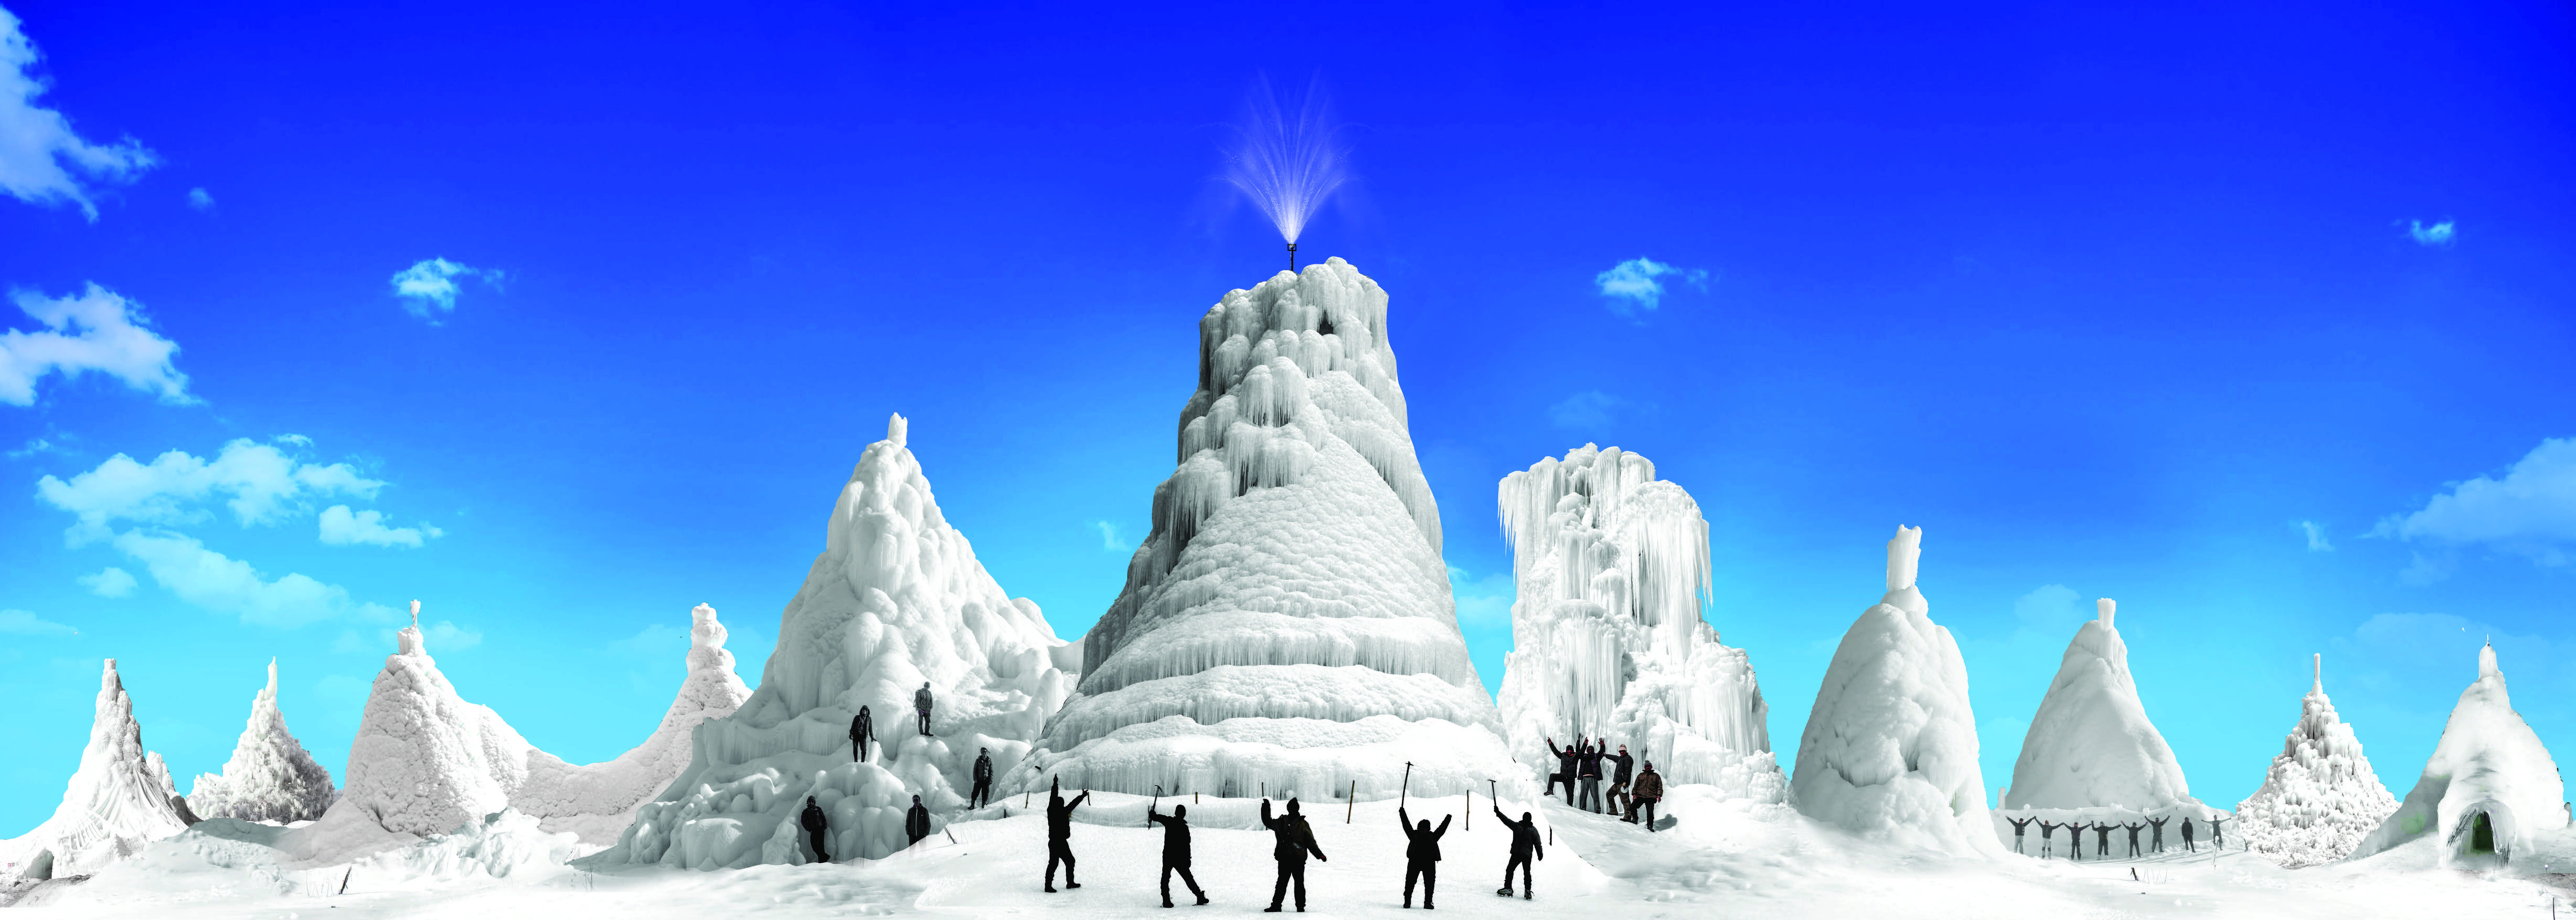
\includegraphics[width=\textwidth]{figs/AIRs_Ladakh}
	\caption{Compilation of AIRs built in different villages of Ladakh.}
	\label{fig:airs_ladakh}
\end{figure}

In paper I and II, an AIR model was designed to resolve AIR surface processes. In paper II, the modelled volume
evolution of AIRs in Indian Himalayas and the Swiss Alps were compared. In paper III, the evolution of AIRs
using different fountain scheduling strategies were compared. The results of these papers can be summarised as
follows:

\begin{enumerate} 

\item Volumes of ice stupas located in different regions may differ by an order of magnitude. The differences
  could be attributed to the accelerated sublimation process in colder and drier regions.

\item Water losses of ice stupas may be upto 80 \% due to excessive water input. However, water supply
  management through fountain scheduling strategies can produce icestupas of similar volumes by using just
  one-tenth of the water supply.

\item Traditional construction systems demand significant maintenance efforts since they are prone to freezing
  events in the fountain pipeline. However, automated construction systems can prevent these events to make the
  construction process maintenance-free.

\end{enumerate}

\section{Discussion}

\subsection{Ice stupas vs Ice terraces}

\begin{table}[htb]
	\begin{tabularx}{\textwidth}{X | X | X | X}
		\hline
    \textbf{Technology}& \textbf{Water storage}& \textbf{Daily meltwater supply (days)}& \textbf{Duration} \\
    \hline
		Ice terraces			& < 30				     & 2 months				\\
    Ice stupas        & < 10             & 5				\\
		\hline
	\end{tabularx}
	\label{tab:table1}
	\caption{This is a caption text.}
\end{table}


\subsection{The state of AIR technology}

This thesis shows one strategy that can improve the water-use efficiency of this technology. This strategy was
chosen as it enabled us to use the AIR model as a tool in a simple and effective manner. With sufficient
engineering expertise, a lot can be done when it comes to the tools used for ice stupa construction. The
fountain nozzle design is crucial for increasing the ice volumes achieved. However, no methodology currently
exists to rank the several fountain nozzles used for construction. An ideal pipeline configuration could make
this technology cheaper and maintenance free. However, optimization of the pipeline material and diameters are
yet to be carried out despite the loss of human hours on pipeline freezing events and the potential cost
reduction possible through use of cheaper pipeline materials and sizes. Therefore, we strongly encourage the
engineering community to get involved and push the limits of the size and survival duration of artificial ice
reservoirs. 

Application on ice terraces

\subsection{Artificial glaciers: A thought experiment}

By definition, all glaciers, including the smallest ones, are bodies of sedimentary ice which were built up by
progressive snow compaction and firnification and flow downhill under the influence of gravity
\cite{benndouglasiGlaciersGlaciation2014}. Hence, because of their genesis and composition, AIRs differ from
glaciers. But when classified in terms of size and survival duration, AIRs exhibit similar characterestics to
very small glaciers. The glossary of glacier mass balance and related terms by
\citet{cogleyGlossaryGlacierMass2010} defines very small glaciers or glacierets as follows:

\begin{thesis_quotation}
  A very small glacier, typically less than 0.25 $km^2$ in extent, with no marked flow pattern
  visible at the surface. To qualify as a glacieret, an ice body must persist for at least two consecutive
  years. Glacierets can be of any shape, and usually occupy sheltered parts of the landscape. Windborne snow and
  avalanches can be dominant contributors to the accumulation of glacierets. 
\end{thesis_quotation}

This rather broad definition of glacierets or very small glaciers may be the one best suited for AIRs. Ice
terraces have been measured to have areas upto 0.15 $km^2$ by
\citet{nusserSociohydrologyArtificialGlaciers2019}. Ice stupas have been observed to last for two consecutive
years. However, most AIRs are neither so large or last so long.

Based on this definition, we can define "artificial glaciers" as ice bodies that are both larger in area and
last longer than two consecutive years. Manmade ice structures can, in theory, occupy any area provided for
their construction. But can AIRs, like glaciers, also survive the summer and compound their size every
consecutive winter? 

\begin{figure}[htb]
  \centering
	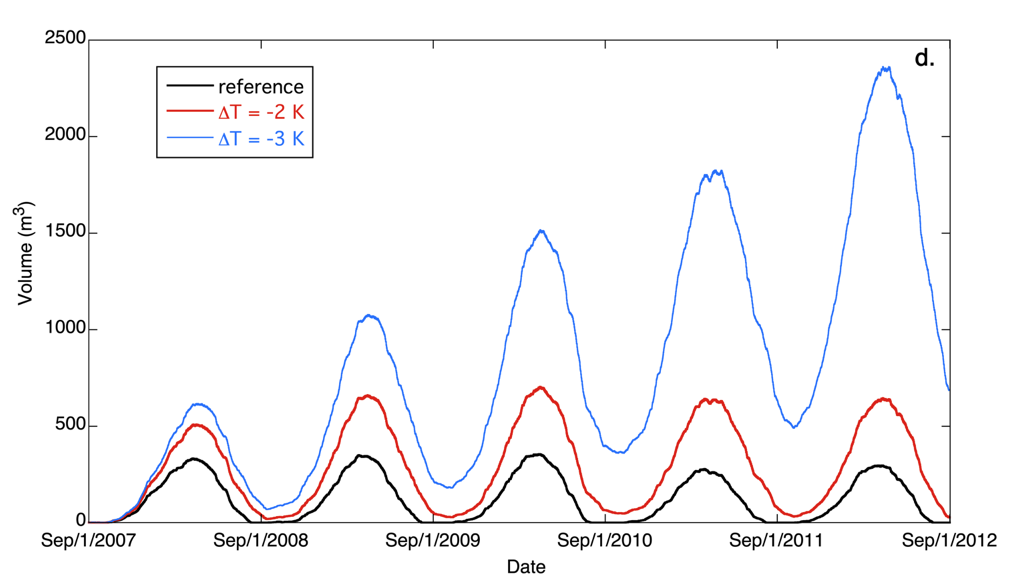
\includegraphics[width=12 cm]{figs/PIR_example.png}
  \caption{The effect of a negative temperature perturbation. For $\Delta T = -3 \degree C$ the icestupa does
  not disappear anymore but is growing from year to year.}
\label{fig:PIR}
\end{figure}

A possible way to study this question is to decrease the air temperature uniformly (temperature change $\Delta
T$). This will imply a stronger negative sensible heat flux in summer, thus accelerating icestupa growth and
slowing down its decay. We found a break-even point for $\Delta T = -2 \degree C$ (Fig. \ref{fig:PIR}). For
larger negative values of $\Delta T$ the icestupa does not disappear in summer and keeps growing from year to
year. For $\Delta T = -3 \degree C$, the maximum volume in the fifth year is about 4 times that in the first
year. Therefore, there exists weather conditions where they can last as long as the water supplies last (see
Fig. \ref{fig:PIR}). Paper III provides the datasets and methodology used to produce these simulations.


\section{Recommendations}

\section{Suggestions for future research}

\begin{itemize} 

\item Identification of favourable locations using AIR suitability and water scarcity index.

\item Cosistupa model development for inspecting ice surface processes.

\end{itemize}

\section{Final thoughts}


% With a special focus on ice stupas, a mass and energy balance model was developed and used as a tool to quantify
% the influence of meteorological conditions and fountain characteristics. The meteorological and fountain
% observations were used as model input; AIR volume observations were used to calibrate the model parameters and
% validate its ice volume estimations.

% The model has been shown to perform excellently when calibrated with the AIR datasets.  It could be shown that
% the maximum volume of AIRs located in the IN and CH regions differ by an order of magnitude. These differences
% were caused by the stronger sublimation process due to the colder and drier weather conditions of the IN region. 

% AIR maintenance requirement was reduced and their fountain freezing events were prevented by developing an
% automated construction strategy. Fountain operation was made 8 times more efficient and effortless through the
% use of an automation system that scheduled discharge rates based on the recommendations of the AIR model. 

% \begin{itemize} 

% \item[\tiny{$\blacksquare$}] Colder, drier and less cloudy construction locations form long-lasting AIRs with
%   higher maximum ice volumes. 

% \item[\tiny{$\blacksquare$}] Weather-sensitive fountain systems produce larger and efficient AIRs effortlessly. 

% \end{itemize}
